\documentclass[12pt,letterpaper]{article}
\usepackage{graphicx,textcomp}
\usepackage{natbib}
\usepackage{setspace}
\usepackage{fullpage}
\usepackage{color}
\usepackage[reqno]{amsmath}
\usepackage{amsthm}
\usepackage{fancyvrb}
\usepackage{amssymb,enumerate}
\usepackage[all]{xy}
\usepackage{endnotes}
\usepackage{lscape}
\newtheorem{com}{Comment}
\usepackage{float}
\usepackage{hyperref}
\newtheorem{lem} {Lemma}
\newtheorem{prop}{Proposition}
\newtheorem{thm}{Theorem}
\newtheorem{defn}{Definition}
\newtheorem{cor}{Corollary}
\newtheorem{obs}{Observation}
\usepackage[compact]{titlesec}
\usepackage{dcolumn}
\usepackage{tikz}
\usetikzlibrary{arrows}
\usepackage{multirow}
\usepackage{xcolor}
\newcolumntype{.}{D{.}{.}{-1}}
\newcolumntype{d}[1]{D{.}{.}{#1}}
\definecolor{light-gray}{gray}{0.65}
\usepackage{url}
\usepackage{listings}
\usepackage{color}

\definecolor{codegreen}{rgb}{0,0.6,0}
\definecolor{codegray}{rgb}{0.5,0.5,0.5}
\definecolor{codepurple}{rgb}{0.58,0,0.82}
\definecolor{backcolour}{rgb}{0.95,0.95,0.92}

\lstdefinestyle{mystyle}{
	backgroundcolor=\color{backcolour},   
	commentstyle=\color{codegreen},
	keywordstyle=\color{magenta},
	numberstyle=\tiny\color{codegray},
	stringstyle=\color{codepurple},
	basicstyle=\footnotesize,
	breakatwhitespace=false,         
	breaklines=true,                 
	captionpos=b,                    
	keepspaces=true,                 
	numbers=left,                    
	numbersep=5pt,                  
	showspaces=false,                
	showstringspaces=false,
	showtabs=false,                  
	tabsize=2
}
\lstset{style=mystyle}
\newcommand{\Sref}[1]{Section~\ref{#1}}
\newtheorem{hyp}{Hypothesis}



\title{Replication Paper - Niall Carty}
\date{Due: March 31, 2024}
\author{Are Irish Voters Moving to the Left? Irish Political Studies \\ \textit{(Stefan Müller, Aidan Regan, 2021)} }



\begin{document}
	\maketitle
	\section*{Introduction}

\vspace{.25cm}
The abstract to this paper notes that the Irish party system has been an outlier in comparative politics. Ireland never had a left-right divide in parliament, and for decades, the dominant centrist political parties competed around a centre-right policy agenda. Müller and Regan note that the absence of an explicit left-right divide in party competition suggested that Irish voters, on average, occupy centre-right policy preferences. \\

\noindent Combining survey data since 1973 and all Irish election studies between 2002 and 2020, the authors aim to show that the average Irish voter now leans to the centre-left. They also state that income has recently emerged as a predictor of left-right self-placement, and that left-right
positions increasingly structure vote choice. Müller and Regan find that these patterns hold when using
policy preferences on taxes, spending, and government interventions to
reduce inequality as alternative indicators. They outline potential explanations
for this leftward shift, and conclude that these developments might be
anchored in economic inequalities and the left populist strategies of Sinn Féin. \\

\noindent The replication of the data behind this paper is presented below, as well as an additional contribution to the work. 


\newpage

\section*{Figure 1} 
\vspace{.25cm}

Average left-right self-placements of Irish voters, 1973–2020, based on various
surveys.

\begin{lstlisting}[language=R]

# load harmonised survey dataset (created in 00a_filter_and_harmonise_lr_surveys.R)

data_surveys_1973_2020 <- readRDS("data_surveys_1973_2020.rds")


# load dataset with harmonised election studies

dat_electionstudies <- readRDS("data_election_studies_ireland.rds")

table(dat_electionstudies$left_right_self,
dat_electionstudies$year)

# descriptive statistics of surveys with Irish respondents, 1973-2020

# filter only Irish respondents
dat_ire <- filter(data_surveys_1973_2020, 
country == "Ireland")


# number of years
length(unique(dat_ire$year))
# 47 years

# number of valid responses from Irish citizens
dat_ire %>% 
filter(!is.na(left_right0to10)) %>% 
filter(!is.na(year)) %>% 
nrow()
# 152344 valid responses


# Sources: CSES, ESS, Eurobarometer
table(dat_ire$dataset)


set.seed(14)
dat_ire_sum <- dat_ire %>%
group_by(year) %>%
do(data.frame(rbind(Hmisc::smean.cl.boot(.$left_right0to10))))


## Figure 1 ----
ggplot(dat_ire_sum, aes(x = year, y = Mean, 
ymin = Lower, ymax = Upper)) +
geom_smooth(fill = "grey80", colour = "black", alpha = 1) + 
geom_point(size = 3, fill = "grey40", colour = "grey40") +
geom_linerange(colour = "grey40") +
scale_x_continuous(breaks = c(seq(1975, 2020, 5))) +
labs(x = "Survey Year", y = "Average Left-Right Self-Placement")
ggsave("fig_01.pdf",
width = 9, height = 5)

 \end{lstlisting}

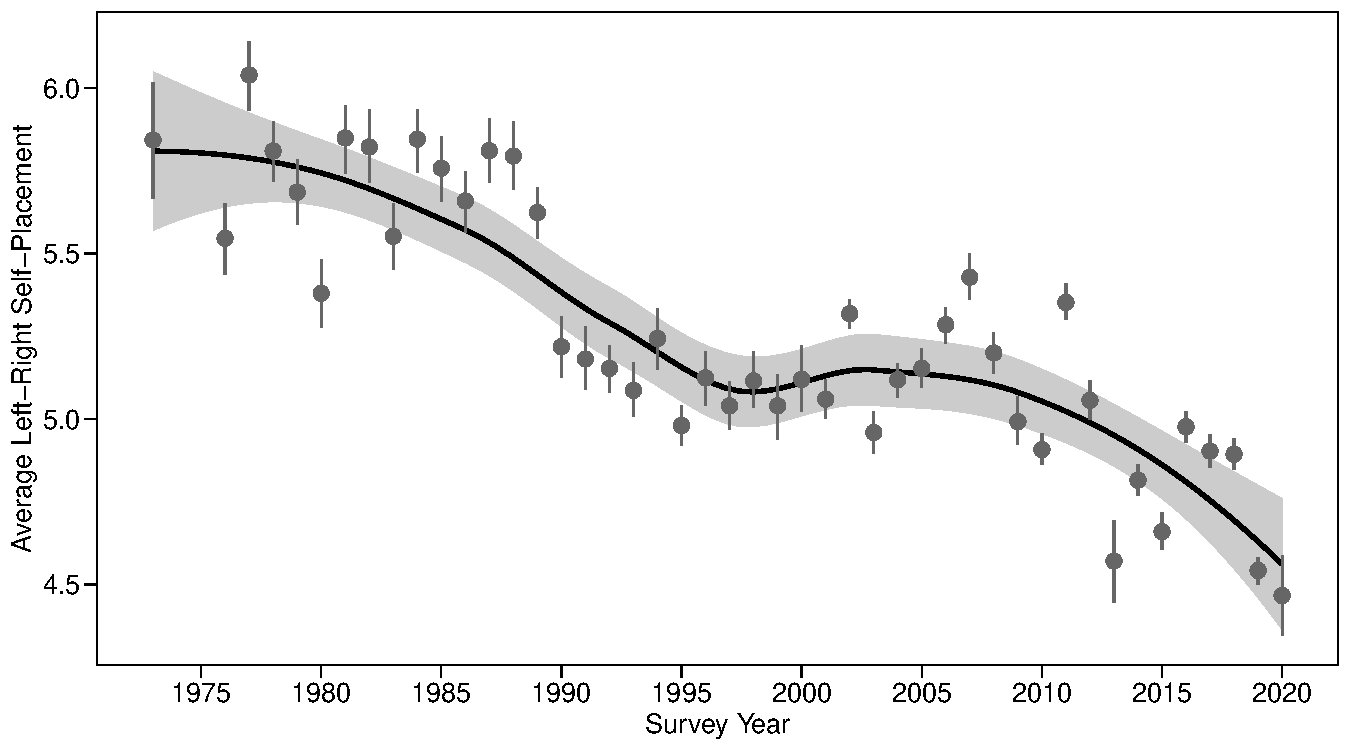
\includegraphics[width=1\textwidth]{fig_01}

\newpage

\section*{Figure 2} 
\vspace{.25cm}

Average-left right self-placements by first-preference vote choice.

\begin{lstlisting}[language=R]
## Figure 2 ----

table(dat_electionstudies$party_vote_recoded_precise,
dat_electionstudies$year)

# select only a subset of parties for Figure 2
dat_all_elections_subset <- dat_electionstudies %>% 
filter(party_vote_recoded_precise %in% c(
"Solidarity PBP",
"Social Democrats", "Sinn Fein",
"Green Party", "Labour Party",
"Fianna Fail", "Fine Gael"
))


left_right_self_partymeans <- dat_all_elections_subset %>%
srvyr::as_survey_design() %>% 
group_by(year, party_vote_recoded_precise) %>%
summarise(lr_mean = srvyr::survey_mean(left_right_self, 
na.rm = TRUE)) %>% 
mutate(lr_ci_95_lower = lr_mean - 1.96 * lr_mean_se) %>% 
mutate(lr_ci_95_upper = lr_mean + 1.96 * lr_mean_se) %>% 
mutate(lr_ci_90_lower = lr_mean - 1.645 * lr_mean_se) %>% 
mutate(lr_ci_90_upper = lr_mean + 1.645 * lr_mean_se) 

# reorder parties
left_right_self_partymeans$party_vote_recoded_precise <- factor(
left_right_self_partymeans$party_vote_recoded_precise,
levels = c("Fine Gael", 
"Fianna Fail",
"Labour Party",
"Green Party", 
"Sinn Fein",
"Social Democrats", 
"Solidarity PBP"))

ggplot(left_right_self_partymeans, 
aes(x = forcats::fct_rev(as.factor(year)), 
y = lr_mean,
colour = party_vote_recoded_precise)) +
geom_point(size = 2) +
# geom_linerange(aes(ymin = lr_ci_90_lower,
#                    ymax = lr_ci_90_upper),
#                size = 1.05) +
geom_linerange(aes(ymin = lr_ci_95_lower,
ymax = lr_ci_95_upper)) +
coord_flip() +
scale_y_continuous(limits = c(0, 10), 
breaks = c(seq(0, 10, 1))) +
scale_colour_manual(values = colours_party) +
facet_grid(party_vote_recoded_precise ~.) +
theme(legend.position = "none",
axis.text.y = element_text(size = 12),
axis.title = element_text(size = 12),
strip.text.y = element_text(angle = 0, hjust = 0, size = 12))  +
labs(x = "Election",  
y = "Average Left-Right Self-Placement")

\end{lstlisting}


\begin{figure}
	\centering
	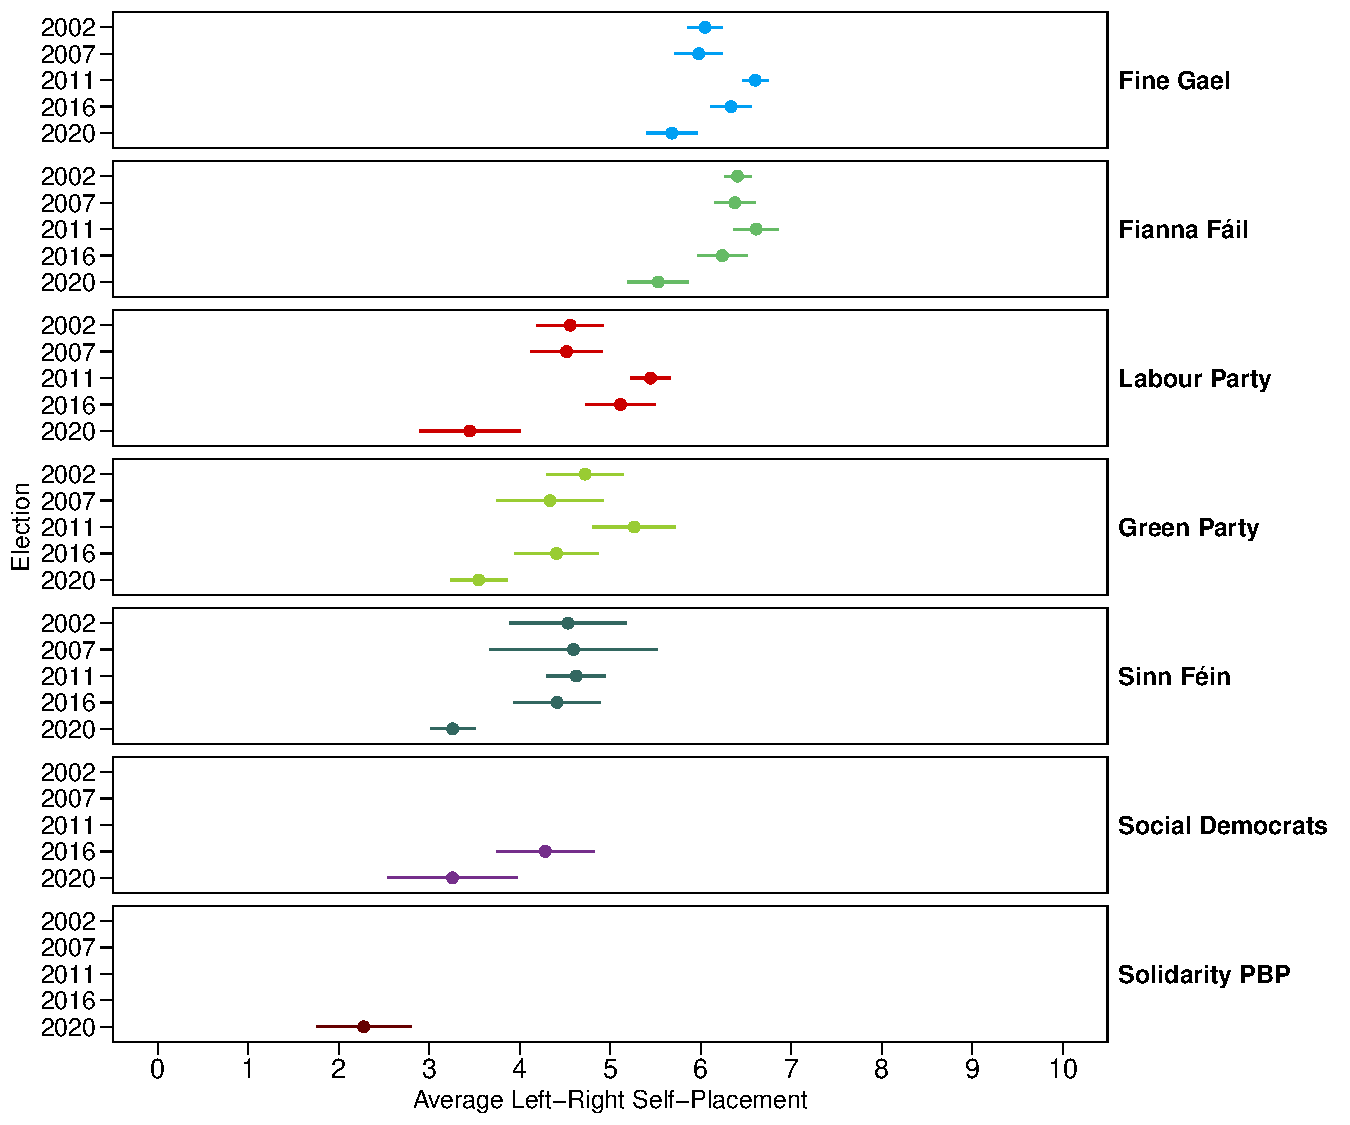
\includegraphics[width=1\linewidth]{fig_02}
	\label{figure 2}
\end{figure}


\newpage
\section*{Table 1: Linear Regression Models} 
\vspace{.25cm}

\begin{lstlisting}[language=R]
	
## Linear regression models ----


dat_reg <- dat_electionstudies

summary(dat_reg)

# adjust factor variables
dat_reg$income_harmonised <- as.factor(dat_reg$income_harmonised)


dat_reg$gender <- relevel(as.factor(dat_reg$gender), 
ref = "Male")
dat_reg$urban <- relevel(as.factor(dat_reg$urban), 
ref= "0")

dat_reg$university_degree <- relevel(as.factor(dat_reg$university_degree), 
ref = "0")

dat_reg$income_harmonised <- relevel(as.factor(dat_reg$income_harmonised), 
ref = "1")

dat_reg$party_vote <- relevel(as.factor(dat_reg$party_vote), 
ref = "Fianna Fail")

dat_reg$age_cat <- factor(dat_reg$age_cat)


# models with left-right self-placements as DV

# 2002
lm_lr_02 <- lm(left_right_self ~ 
income_harmonised  +
age_cat +
gender + urban +
university_degree,
weight = weights,
data = filter(dat_reg,
year == "2002"))

# 2007
lm_lr_07 <- update(lm_lr_02,  
data = filter(dat_reg,
year == "2007"))

# 2011
lm_lr_11 <- update(lm_lr_02,  
data = filter(dat_reg,
year == "2011"))

# 2011
lm_lr_16 <- update(lm_lr_02,  
data = filter(dat_reg,
year == "2016"))


# 2020
lm_lr_20 <- update(lm_lr_02,  
data = filter(dat_reg,
year == "2020"))

## Table 1 ----
screenreg(list(
lm_lr_02,
lm_lr_07,
lm_lr_11,
lm_lr_16,
lm_lr_20
))

wordreg(list(lm_lr_02,
lm_lr_07,
lm_lr_11,
lm_lr_16,
lm_lr_20),
single.row = FALSE,
custom.coef.names = c(
"(Intercept)",
"Income category: 2 (ref.: 1)",
"Income category: 3",
"Income category: 4",
"Income category: 5",
"Age: 25-34 (ref.: 18-24)",
"Age: 35-44",
"Age: 45-54",
"Age: 55-64",
"Age: 65+",
"Female",
"Urban constituency",
"University degree"),
size = "footnotesize",
custom.model.names = c("2002", "2007", "2011", "2016", "2020"),
file = "tab_01.doc")
\end{lstlisting}

\begin{figure}
	\centering
	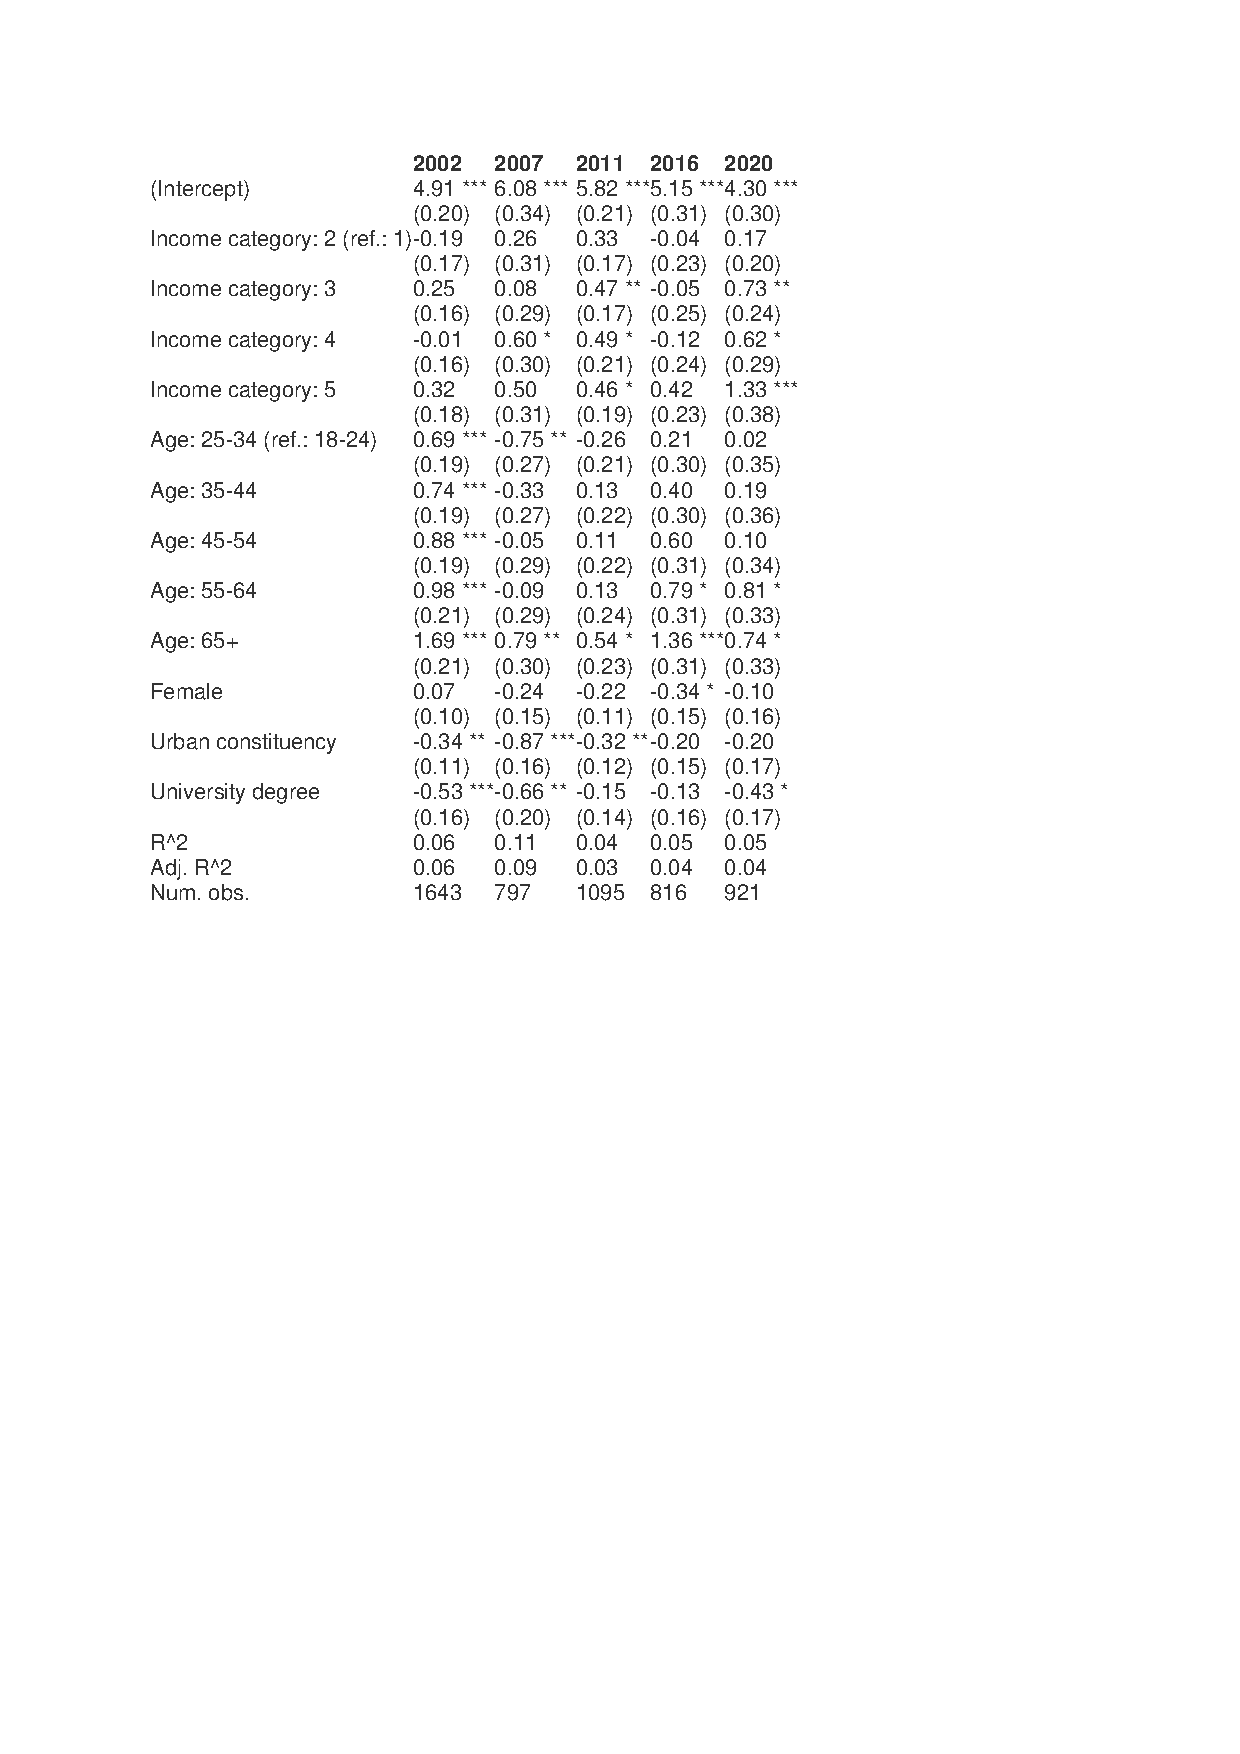
\includegraphics[width=1.5\linewidth]{tab_01.doc}
	\label{fig:tab01}
	
\end{figure}

\newpage
\section*{Figure 3} 
\vspace{.25cm}

 Predicting left-right self-placement conditional on income

\begin{lstlisting}[language=R]

## Figure 3 ----
## get expected values of income levels for each election

# 2002
pred_income_02 <- ggpredict(lm_lr_02, terms = c("income_harmonised"),
condition = c(
age_cat = "35-44",
gender = "Male",
urban = "0",
university_degree = "0")) %>% mutate(model = "2002")
pred_income_02


# 2007
pred_income_07 <- ggpredict(lm_lr_07, terms = c("income_harmonised"),
condition = c(
age_cat = "35-44",
gender = "Male",
urban = "0",
university_degree = "0")) %>% mutate(model = "2007")

pred_income_07

# 2011
pred_income_11 <- ggpredict(lm_lr_11, terms = c("income_harmonised"),
condition = c(
age_cat = "35-44",
gender = "Male",
urban = "0",
university_degree = "0")) %>% mutate(model = "2011")
pred_income_11


# 2016
pred_income_16 <- ggpredict(lm_lr_16, terms = c("income_harmonised"),
condition = c(
age_cat = "35-44",
gender = "Male",
urban = "0",
university_degree = "0")) %>% mutate(model = "2016")
pred_income_16

# 2020
pred_income_20 <- ggpredict(lm_lr_20, terms = c("income_harmonised"),
condition = c(
age_cat = "35-44",
gender = "Male",
urban = "0",
university_degree = "0")) %>% mutate(model = "2020")
pred_income_20

# bind expected values from all models
pred_income <- bind_rows(pred_income_02,
pred_income_07,
pred_income_11,
pred_income_16,
pred_income_20)

pred_income <- pred_income %>% 
filter(!is.na(x))

# Change labels of income categories
#pred_income <- pred_income %>% 
#mutate(income_cat = dplyr::recode(
# x, "1" = "1: Lowest", "5" = "5: Highest"
# ))

ggplot(pred_income, aes(x = predicted, y = x)) +
geom_point(size = 3) +
geom_errorbarh(aes(xmin = predicted - 1.96 * std.error,
xmax = predicted + 1.96 * std.error),
size = 0.5, height = 0) +
# geom_errorbarh(aes(xmin = predicted - 1.645 * std.error,
#                    xmax = predicted + 1.645 * std.error),
#                size = 1.3, height = 0) +
coord_flip() +
facet_wrap(~model, nrow = 1) +
scale_x_continuous(limits = c(3, 8)) +
labs(x = "Expected Left-Right Self-Placement",
y = "Income Category (from Lowest to Highest)")
ggsave("fig_03.pdf", 
width = 9, height = 5)	
\end{lstlisting}

\begin{figure}
	\centering
	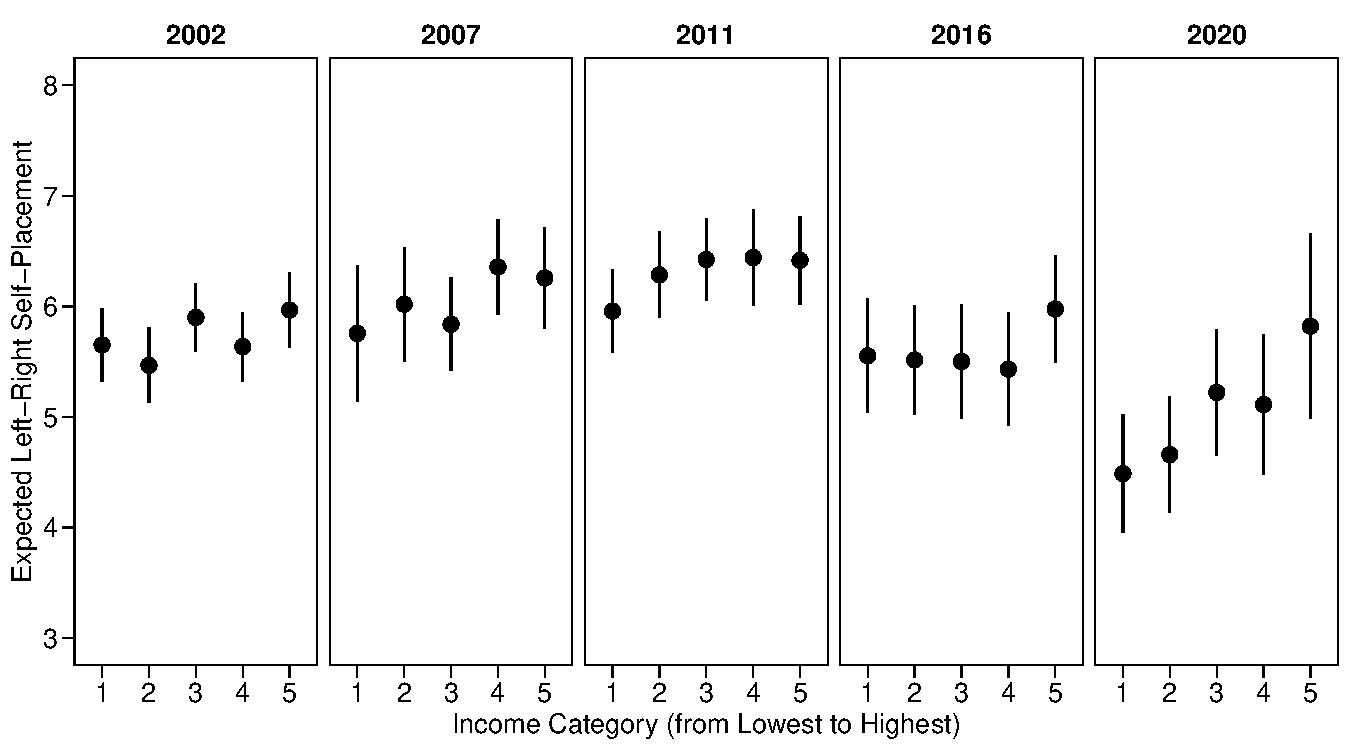
\includegraphics[width=0.8\linewidth]{fig_03}

\end{figure}


\newpage

\section*{Figure 4} 
\vspace{.25cm}

 Predicting vote choice conditional on left-right self-placements

\begin{lstlisting}[language=R]

## Multinomial regression models ----

## predict party choice conditional on left-right self-placement

# get years
years <- unique(dat_reg$year)

# empty dataframe to store predicted probabilities
dat_multinom_merged <- data.frame()

for (i in years) {
	
	dat_year <- filter(dat_reg, year == i)
	
	lm_multinom <- multinom(party_vote ~ left_right_self + income_harmonised + age_cat  + 
	gender + 
	urban + university_degree,
	weight = weights,
	data = dat_year)
	
	aic_election <- lm_multinom$AIC
	dat_effect_lr <- as.data.frame(
	Effect(c("left_right_self"), 
	lm_multinom, xlevels = 20))
	
	dat_effect_lr_prob <- dat_effect_lr %>% 
	select(c(left_right_self, starts_with("prob.")))
	
	dat_effect_lr_prob_long <- dat_effect_lr_prob %>% 
	gather(party_vote_aggregated, predicted, -c(left_right_self)) %>% 
	mutate(party_vote_aggregated = str_replace_all(party_vote_aggregated, "prob.", ""))
	
	
	dat_effect_lr_se <- dat_effect_lr %>% 
	select(c(left_right_self, starts_with("se.prob.")))
	
	dat_effect_lr_se_long <- dat_effect_lr_se %>% 
	gather(party_vote_aggregated, std.error, -c(left_right_self)) %>% 
	mutate(party_vote_aggregated = str_replace_all(party_vote_aggregated, "se.prob.", ""))
	
	dat_effect_lr_se_long <- left_join(dat_effect_lr_prob_long,
	dat_effect_lr_se_long,
	by = c("party_vote_aggregated", "left_right_self")) %>% 
	mutate(party_vote_aggregated = str_replace_all(party_vote_aggregated, "\\.", " ")) 
	
	dat_effect_lr_se_long$year <- i
	dat_effect_lr_se_long$aic_election <- aic_election
	
	dat_multinom_merged <- bind_rows(dat_effect_lr_se_long,
	dat_multinom_merged)
	}

# colours for parties and levels for factors
colours_party <- c("#66BB66", "#009FF3", "#326760",
"red",
"grey70")

factors_party <- c("Fianna Fail", "Fine Gael",
"Sinn Fein",
"Greens and Left bloc",
"Other and Independents")

dat_multinom_merged$party_vote_aggregated <- factor(dat_multinom_merged$party_vote_aggregated,
levels = factors_party)

# determine confidence intervals
ci_90 <- 1.645
ci_95 <- 1.96

## Figure 4 ----
ggplot(dat_multinom_merged, aes(x = left_right_self, 
y = predicted)) +
# geom_ribbon(aes(ymin = predicted - ci_90 * std.error,
#                 ymax = predicted + ci_90 * std.error,
#                 fill = party_vote_aggregated)) +
geom_ribbon(aes(ymin = predicted - ci_95 * std.error,
ymax = predicted + ci_95 * std.error,
fill = party_vote_aggregated)) +
geom_line() +
scale_fill_manual(values = colours_party) +
scale_x_continuous(breaks = c(seq(0, 10, 2))) +
scale_colour_grey(name = "Income", start = 0.7, end = 0) +
facet_grid(party_vote_aggregated~year, scales = "free_x", 
labeller = label_wrap_gen(width = 15)) +
labs(x = "Left-right self-placement", y = "Pr(Party as First-Preference Vote Choice)") +
theme(legend.position = "none", 
legend.title = element_blank())
ggsave("fig_04.pdf", 
width = 9, height = 10)

	
\end{lstlisting}

\begin{figure}
	\centering
	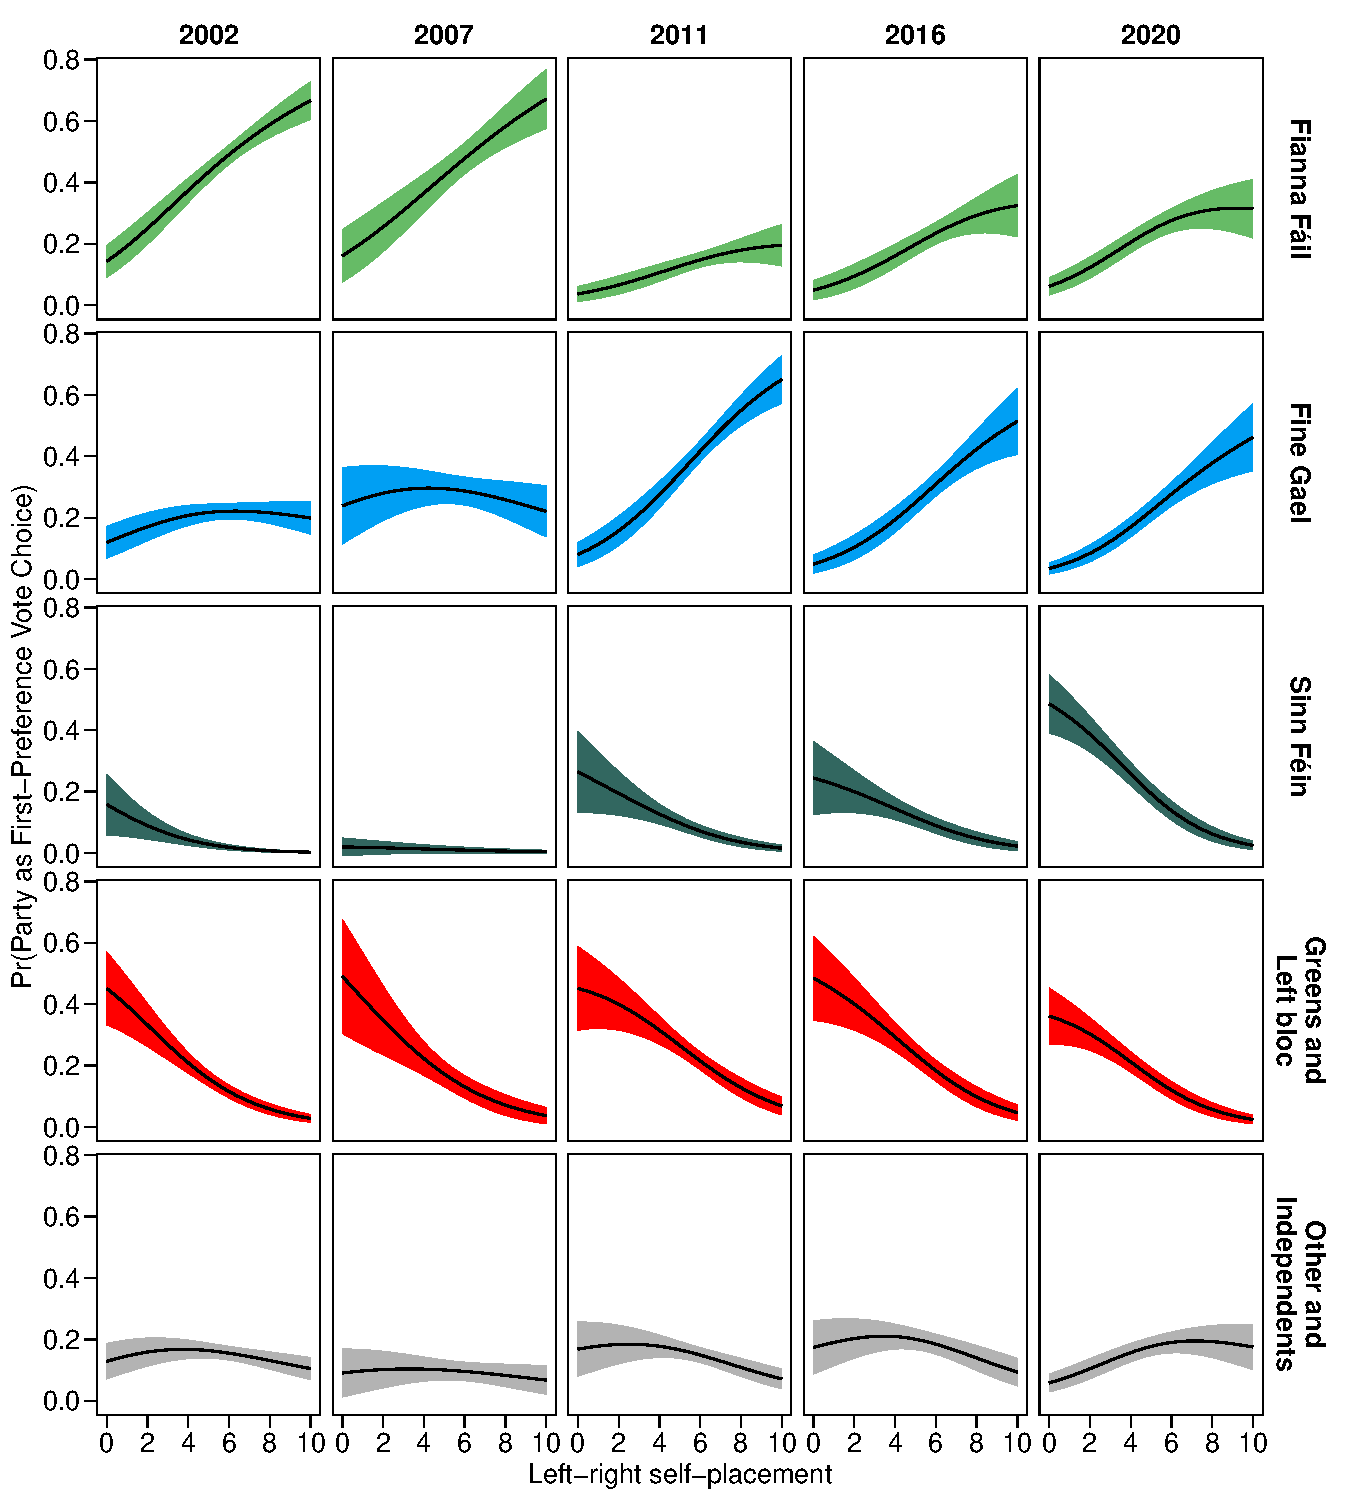
\includegraphics[width=0.9\linewidth]{fig_04}
\end{figure}


\newpage
\section*{Figure 5} 
\vspace{.25cm}

Predicting vote choice in the 2020 general election conditional on attitudes
towards reducing differences in income and wealth.

\begin{lstlisting}[language=R]
## Repeat multinomial logistic regression models for 2020 with different set of independent variables

dat_reg_multinom <- dat_reg
head(dat_reg_multinom)

multinom_20_incomediff <- multinom(party_vote ~ income_differences + income_harmonised + 
age_cat  + 
gender + 
urban + university_degree,
weight = weights,
data = filter(dat_reg_multinom, 
year == "2020"))

multinom_20_incomediff

multinom_20_taxespend <- multinom(party_vote ~ taxes_spending + 
income_harmonised +
age_cat  + 
gender +  
urban + university_degree,
weight = weights,
data = filter(dat_reg_multinom, 
year == "2020"))

# get predicted probabilities for income differences
dat_effect_incomediff_2020 <- as.data.frame(
Effect(c("income_differences"), 
multinom_20_incomediff, xlevels = 20))

dat_effect_incomediff_2020_prob <- dat_effect_incomediff_2020 %>% 
select(c(income_differences, starts_with("prob.")))

dat_effect_incomediff_prob_2020_long <- dat_effect_incomediff_2020_prob %>% 
gather(party_vote_aggregated, predicted, -c(income_differences)) %>% 
mutate(party_vote_aggregated = str_replace_all(party_vote_aggregated, "prob.", ""))

dat_effect_incomediff_2020_se <- dat_effect_incomediff_2020 %>% 
select(c(income_differences, starts_with("se.prob.")))

dat_effect_incomediff_se_2020_long <- dat_effect_incomediff_2020_se %>% 
gather(party_vote_aggregated, std.error, -c(income_differences)) %>% 
mutate(party_vote_aggregated = str_replace_all(party_vote_aggregated, "se.prob.", ""))

dat_effect_incomediff_2020_se_long <- left_join(dat_effect_incomediff_prob_2020_long,
dat_effect_incomediff_se_2020_long,
by = c("party_vote_aggregated", "income_differences")) %>% 
mutate(party_vote_aggregated = str_replace_all(party_vote_aggregated, "\\.", " ")) 

dat_effect_incomediff_2020_se_long$party_vote_aggregated <- 
factor(dat_effect_incomediff_2020_se_long$party_vote_aggregated,
levels = factors_party)

# colours for parties and levels for factors
colours_party <- c("#66BB66", "#009FF3", "#326760", "red", "grey70")

## Figure 5 ----
ggplot(dat_effect_incomediff_2020_se_long, aes(x = income_differences, 
y = predicted)) +
# geom_ribbon(aes(ymin = predicted - ci_90 * std.error,
#                 ymax = predicted + ci_90 * std.error,
#                 fill = party_vote_aggregated)) +
geom_ribbon(aes(ymin = predicted - ci_95 * std.error,
ymax = predicted + ci_95 * std.error,
fill = party_vote_aggregated)) +
geom_line() +
scale_fill_manual(values = colours_party) +
scale_x_continuous(breaks = c(seq(0, 10, 2))) +
scale_colour_grey(name = "Income", start = 0.7, end = 0) +
facet_wrap(~party_vote_aggregated,
labeller = label_wrap_gen(width = 15),
nrow = 1) +
scale_y_continuous(limits = c(0, 0.6),
breaks = c(seq(0, 0.6, 0.1))) +  
labs(x = "Reduce Differences in Income and Wealth", y = "Pr(Party as First-Preference Vote Choice)") +
theme(legend.position = "none", 
legend.title = element_blank())
ggsave("fig_05.pdf",
width = 9, height = 4.5)
\end{lstlisting}

\begin{figure}
	\centering
	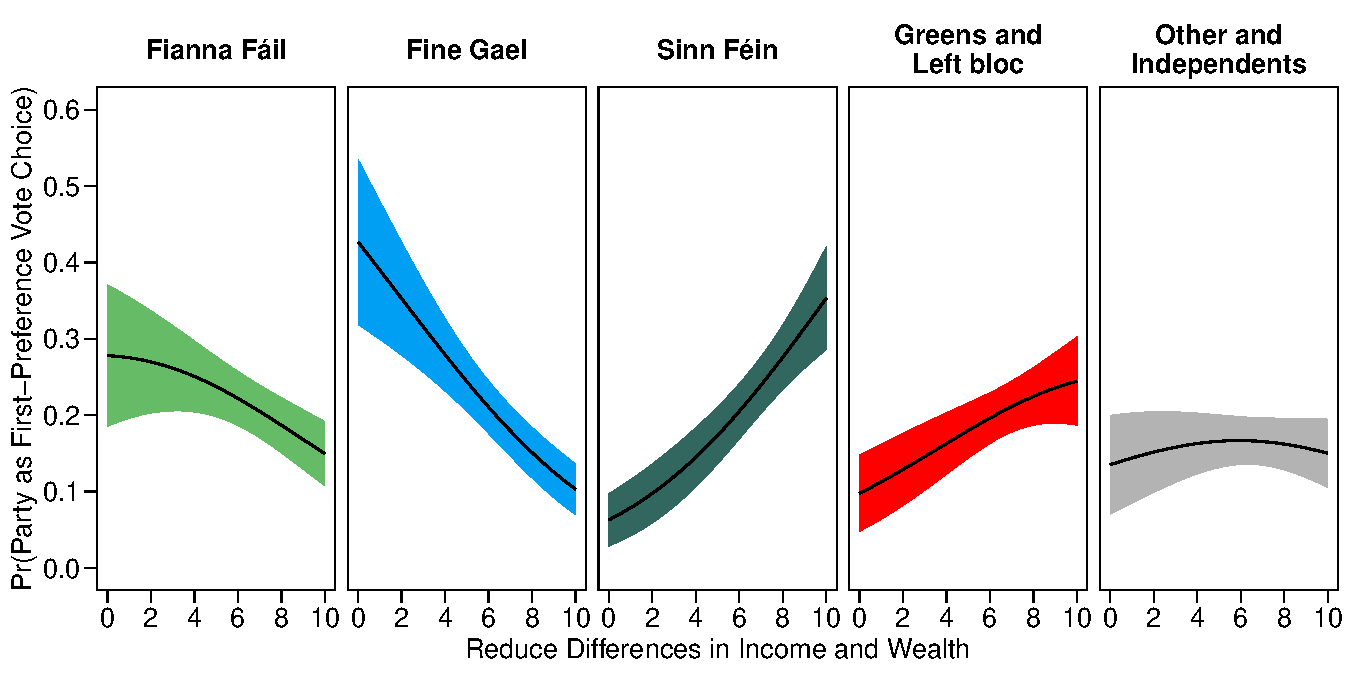
\includegraphics[width=0.8\linewidth]{fig_05}
\end{figure}

\newpage
\section*{Figure 6} 
\vspace{.25cm}

Figure 6. Predicting vote choice in the 2020 general election conditional on attitudes
towards taxes and spending.

\begin{lstlisting}[language=R]
# get predicted values for taxes and spending
dat_effect_tax_2020 <- as.data.frame(
Effect(c("taxes_spending"), 
multinom_20_taxespend, xlevels = 20))

dat_effect_tax_2020_prob <- dat_effect_tax_2020 %>% 
select(c(taxes_spending, starts_with("prob.")))

dat_effect_tax_prob_2020_long <- dat_effect_tax_2020_prob %>% 
gather(party_vote_aggregated, predicted, -c(taxes_spending)) %>% 
mutate(party_vote_aggregated = str_replace_all(party_vote_aggregated, "prob.", ""))

dat_effect_tax_2020_se <- dat_effect_tax_2020 %>% 
select(c(taxes_spending, starts_with("se.prob.")))

dat_effect_tax_se_2020_long <- dat_effect_tax_2020_se %>% 
gather(party_vote_aggregated, std.error, -c(taxes_spending)) %>% 
mutate(party_vote_aggregated = str_replace_all(party_vote_aggregated, "se.prob.", ""))

dat_effect_tax_2020_se_long <- left_join(dat_effect_tax_prob_2020_long,
dat_effect_tax_se_2020_long,
by = c("party_vote_aggregated", "taxes_spending")) %>% 
mutate(party_vote_aggregated = str_replace_all(party_vote_aggregated, "\\.", " ")) 



dat_effect_tax_2020_se_long$party_vote_aggregated <- 
factor(dat_effect_tax_2020_se_long$party_vote_aggregated,
levels = factors_party)

library(shades)

## Figure 6 ----
ggplot(dat_effect_tax_2020_se_long, aes(x = taxes_spending, 
y = predicted)) +
# geom_ribbon(aes(ymin = predicted - ci_90 * std.error,
#                 ymax = predicted + ci_90 * std.error,
#                 fill = party_vote_aggregated)) +
geom_ribbon(aes(ymin = predicted - ci_95 * std.error,
ymax = predicted + ci_95 * std.error,
fill = party_vote_aggregated)) +
geom_line() +
scale_fill_manual(values = colours_party) +
scale_x_continuous(breaks = c(seq(0, 10, 2))) +
scale_colour_grey(name = "Income", start = 0.7, end = 0) +
facet_wrap(~party_vote_aggregated,
labeller = label_wrap_gen(width = 15),
nrow = 1) +
scale_y_continuous(limits = c(0, 0.6),
breaks = c(seq(0, 0.6, 0.1))) +
labs(x = "More Taxes and Spending", y = "Pr(Party as First-Preference Vote Choice)") +
theme(legend.position = "none", 
legend.title = element_blank())
ggsave("fig_06.pdf",
width = 9, height = 4.5)

\end{lstlisting}

\begin{figure}
	\centering
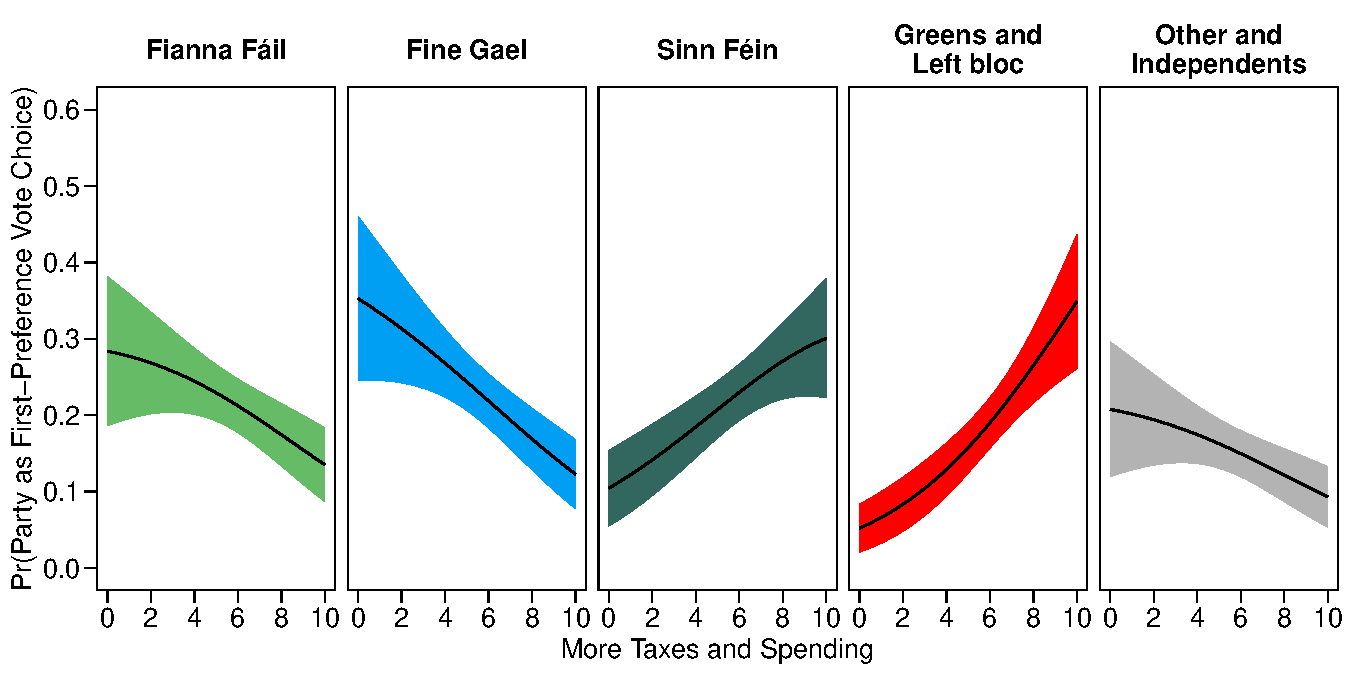
\includegraphics[width=0.9\linewidth]{fig_06}
\end{figure}

\newpage
\section*{Twist} 
\vspace{.25cm}

Added “Urban” as an interaction term to each of the linear regression models for 2020.\\

\noindent Why? The authors note that “Urban cities with a concentration of high-growth multinationals tend to have rapidly growing house prices, high levels of market income inequalities, and very unequal access to housing wealth”, so appears to be a variable of particular interest.

\begin{lstlisting}[language=R]
	
	# Model with interaction term for taxes and spending
	lm_taxesspend_Int_20 <- lm(taxes_spending ~ urban * age_cat +
	gender + university_degree + urban * income_harmonised,
	weight = weights,
	data = filter(dat_reg, year == "2020"))
	
	lm_taxesspend_Int_20 
	
	# Model with interaction term for income differences
	lm_incomediff__Int_20 <- lm(income_differences ~ urban * age_cat +
	gender + university_degree + urban * income_harmonised,
	weight = weights,
	data = filter(dat_reg, year == "2020"))
	
	lm_incomediff__Int_20
	
	lm_lr_02 <- lm(left_right_self ~ 
	income_harmonised  +
	age_cat +
	gender + urban +
	university_degree,
	weight = weights,
	data = filter(dat_reg,
	year == "2002"))
	
	lm_lr_20 <- update(lm_lr_02,  
	data = filter(dat_reg,
	year == "2020"))
	
	lm_lr_urban_INT <- lm(left_right_self ~ 
	urban * income_harmonised  +
	urban * age_cat +
	gender + university_degree,
	weight = weights,
	data = filter(dat_reg, year == "2020"))
	
	lm_lr_urban_INT
	
\end{lstlisting}


\begin{figure}
	\centering
	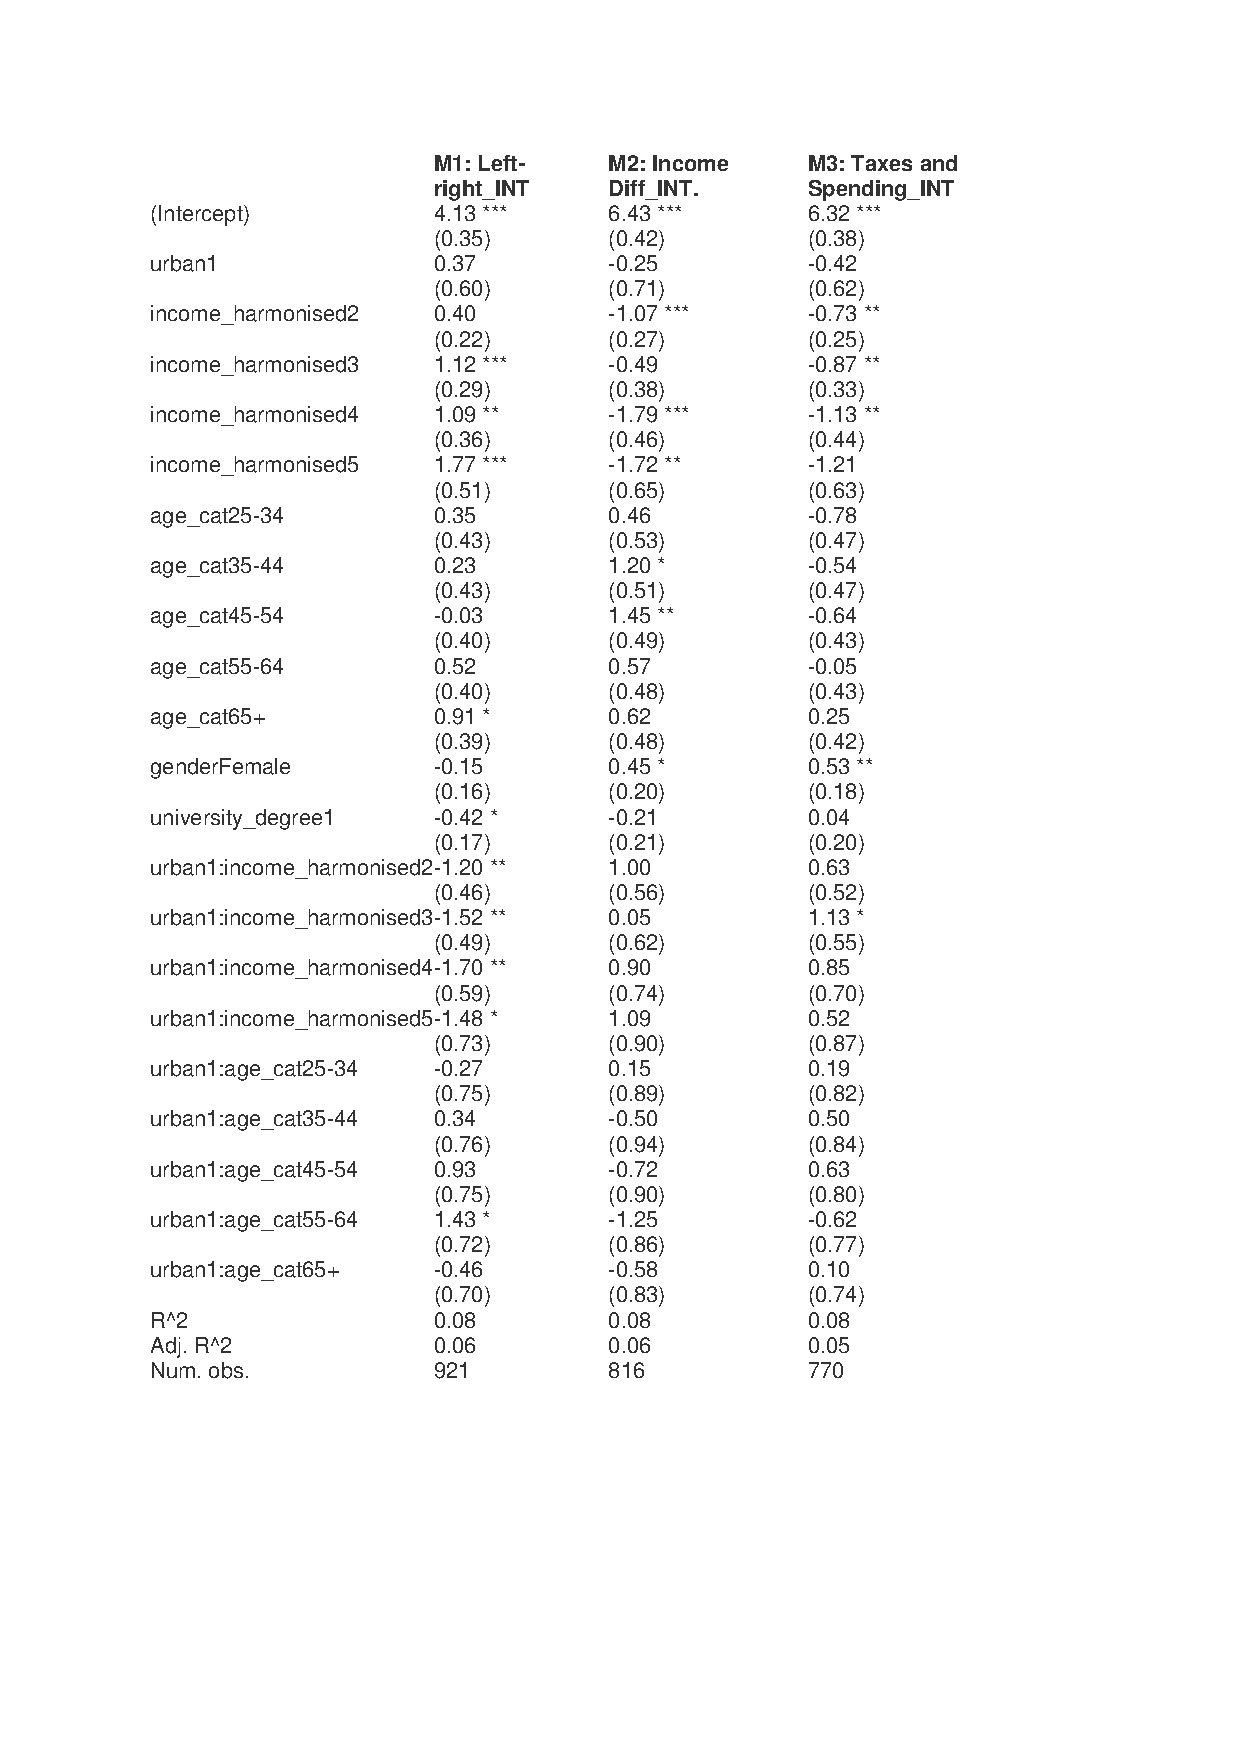
\includegraphics[width=1\linewidth]{tab_a01INT_PDF.doc}
	\caption{}
	\label{fig:taba01intpdf}
\end{figure}

\newpage
\noindent The results show that the interactions between urban and each of the income categories are significant, as is the interaction of urban and the age category 55-64.\\

\noindent To further explore this relationship, an Anova test was run for each model. Only the addition of the interaction term in the first model appears to have a significant on average affect. 

\begin{lstlisting}[language=R]
	
> anova(lm_lr_20, lm_lr_urban_INT)
Analysis of Variance Table

Model 1: left_right_self ~ income_harmonised + age_cat + gender + urban + 
university_degree
Model 2: left_right_self ~ urban * income_harmonised + urban * age_cat + 
gender + university_degree
Res.Df    RSS Df Sum of Sq      F    Pr(>F)    
1    908 4714.9                                  
2    899 4564.5  9    150.37 3.2907 0.0005876 ***
---

> anova(lm_taxesspend_20, lm_taxesspend_Int_20)
Analysis of Variance Table

Model 1: taxes_spending ~ gender + urban + university_degree + age_cat + 
income_harmonised
Model 2: taxes_spending ~ urban * age_cat + gender + university_degree + 
urban * income_harmonised
Res.Df    RSS Df Sum of Sq      F Pr(>F)
1    757 4124.1                           
2    748 4058.6  9    65.537 1.3421 0.2112
> anova(lm_incomediff_20, lm_incomediff__Int_20)
Analysis of Variance Table

Model 1: income_differences ~ +age_cat + income_harmonised + gender + 
urban + university_degree
Model 2: income_differences ~ urban * age_cat + gender + university_degree + 
urban * income_harmonised
Res.Df    RSS Df Sum of Sq      F Pr(>F)
1    803 5481.9                           
2    794 5414.3  9    67.558 1.1008 0.3595
\end{lstlisting}

\vspace{2cm}
\noindent \textbf{Conclusion}: In the case of Left-Right preferences, the addition of the 'Urban' interaction term for the first model appears to have a significant effect with regard to left wing preferences across all income categories, and also for the 55-64 year old age category, with Urban voters more inclined to vote Left.

\newpage


\end{document}